\section{Music theory}
  This section contains some basic music theory relevant for understanding how music is constructed. It is not necessary to understand everything in depth, but familiarity with these concepts will be of great help when reading the musical parts of the thesis. Throughout the thesis there are several examples and figures using musical notation, so a basic understanding of how to read them is beneficial.

  \subsection{Notes}
    The very core of music is sound. Sounds are vibrations in air which we interpret as pitches if the oscillation is somewhat stable. In the western system the standard reference pitch is \musPitch{A}{4}, which is $440$ Hz. The subscript four indicates the fourth octave. All other pitches are tuned in relation to this reference.

    The musical note is represented on the staff by a circular symbol called the note-head. The vertical placement of the note-head on the staff determines which pitch it represents. This is illustrated in Figure~\ref{fig:piano-notes}, where we can see the placement of the notes from \musPitch{C}{2} up to \musPitch{C}{5}. Notice how only the white keys from the piano are notated directly. The black keys are notated with the \musSharp- and \musFlat-symbols. The \musSharp-symbol is pronounced "sharp" and raises the note by a semitone, and the \musFlat-symbol is pronounced "flat" and lowers the note by a semitone\footnote{a semitone is the smallest musical interval and it is the distance between two adjacent notes}. The horizontal placement is not directly an indication of time or duration; the temporal aspect is instead defined symbolically. The note can also have a stem, which is a vertical line attached to the note-head. The direction of the stem (up or down) does not change the pitch, but it can affect the visual layout of the music.

    \begin{figure}[h]
      \begin{center}
        
\includegraphics[trim={0.8cm 8cm 1.1cm 3.1cm}, clip, width=1\textwidth]{figures/04theory/Piano-notes.pdf}
      \end{center}
      \caption{Overview of note placement on the staff and piano.}\label{fig:piano-notes}
    \end{figure}

    The same musical pitch can be written in several different ways in order to indicate the duration of the note. This is done by using variations of the stem and notehead. In Figure~\ref{fig:note-value} the different parts of the note are highlighted with colour. The note-head is black, and its placement decides which musical pitch is represented. The stem can go either up or down; this does not change the meaning, it only makes the notation more compact when the note is placed high or low on the staff. The direction of the stem can also carry meaning if two notes occur simultaneously on one staff, since it usually indicates two different voices.
    Next we have the beams and the flags coloured in purple and blue respectively. These two carry the same meaning: one flag is equivalent to one beam, meaning they represent the same duration. The beam simply makes the notation less visually crowded when reading.
    The duration symbolized by the flag and beam can be seen in Table~\ref{tab:note-values} and Figure~\ref{fig:notevalues}. These are not exhaustive, since we can alter these durations in several ways, but they are sufficient for the scope of this thesis.

    \begin{figure}[h] % Note values
      \begin{center}
        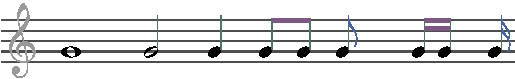
\includegraphics[trim={1cm 0cm 0cm 0cm}, clip, width=0.95\textwidth]{examples/04theory/09-value.cropped.pdf}
      \end{center}
      \caption{The figure shows the parts of the musical note. The note-head in black, stem in green, beam in purple and flag in blue.}\label{fig:note-value}
    \end{figure}

    \begin{table}[h] % Table note values
      \NewDocumentCommand{\musWholeRest} {}{\musFont{\symbol{11}}}
      \NewDocumentCommand{\musHalfRest} {}{\musFont{\symbol{10}}}
      \NewDocumentCommand{\musQuarterRest} {}{\musFont{\symbol{62}}}
      \NewDocumentCommand{\musEightRest} {}{\musFont{\symbol{63}}}
      \NewDocumentCommand{\musSixteenthRest} {}{\musFont{\symbol{64}}}
      \NewDocumentCommand{\musThirtySecondRest} {}{\musFont{\symbol{65}}}
      \caption{Table with common note values, their names and their corresponding duration.}\label{tab:note-values}
      \begin{center}
        \begin{tabular}[c]{|c|l|c|l|}
          \hline
          \multicolumn{1}{|c|}{\textbf{Symbol}} & 
          \multicolumn{1}{c|}{\textbf{Name}} & 
          \multicolumn{1}{c|}{\textbf{Rest symbol}} & 
          \multicolumn{1}{c|}{\textbf{Duration}} \\
          \hline
          \musWhole & Whole note & \musWholeRest & 4 beats \\
          \musHalf & Half note & \musHalfRest & 2 beats \\
          \musQuarter & Quarter note & \musQuarterRest & 1 beat\\
          \musEighth & Eighth note & \musEightRest & $\sfrac{1}{2}$ beat\\
          \musSixteenth & Sixteenth note & \musSixteenthRest & $\sfrac{1}{4}$ beat\\
          \musThirtySecond & Thirty-second note & \musThirtySecondRest & $\sfrac{1}{8}$ beat\\
          \hline
        \end{tabular}
      \end{center}
    \end{table}

    \begin{figure}[h] % Note values tree
      \begin{center}
      \begin{tikzpicture}[
        every node/.style={inner sep=2pt, scale=2},
        level1/.style={yshift=-2cm},
        level2/.style={yshift=-4cm},
        level3/.style={yshift=-6cm},
        every path/.style={->, shorten >=5pt, shorten <=5pt}]

        % --- Top ---
        \node (top) at (0,0) {\musWhole};

        % --- Level 2 ---
        \node (l2a) at (-2,-1) {\musHalf};
        \node (l2b) at ( 2,-1) {\musHalf};

        % --- Level 3 (spread evenly!) ---
        \node (l3a) at (-3,-3) {\musQuarter};
        \node (l3b) at (-1,-3) {\musQuarter};
        \node (l3c) at ( 1,-3) {\musQuarter};
        \node (l3d) at ( 3,-3) {\musQuarter};

        % --- Level 4 (8 notes, evenly spaced) ---
        \node (l4a) at (-3.5,-5) {\musEighth};
        \node (l4b) at (-2.5,-5) {\musEighth};
        \node (l4c) at (-1.5,-5) {\musEighth};
        \node (l4d) at (-0.5,-5) {\musEighth};
        \node (l4e) at ( 0.5,-5) {\musEighth};
        \node (l4f) at ( 1.5,-5) {\musEighth};
        \node (l4g) at ( 2.5,-5) {\musEighth};
        \node (l4h) at ( 3.5,-5) {\musEighth};

        % --- Arrows ---
        \draw[->] (top) -- (l2a);
        \draw[->] (top) -- (l2b);

        \draw[->] (l2a) -- (l3a);
        \draw[->] (l2a) -- (l3b);
        \draw[->] (l2b) -- (l3c);
        \draw[->] (l2b) -- (l3d);

        \draw[->] (l3a) -- (l4a);
        \draw[->] (l3a) -- (l4b);

        \draw[->] (l3b) -- (l4c);
        \draw[->] (l3b) -- (l4d);

        \draw[->] (l3c) -- (l4e);
        \draw[->] (l3c) -- (l4f);

        \draw[->] (l3d) -- (l4g);
        \draw[->] (l3d) -- (l4h);

      \end{tikzpicture}
      \end{center}
      \caption{Tree structure showing how the whole note can be divided into smaller note values. Each level in the tree takes the same amount of time, meaning the whole note at the top lasts as long as the eight eighth notes at the bottom.}
      \label{fig:notevalues}
    \end{figure}

  \subsection{Scales and Keys}\label{sec:keys}
    The musical scale is a building block for creating not only melodies but also harmony, which we will cover a bit later.
    Firstly, a musical scale is an ordered set of musical notes. In the western canon this is usually seven notes. You can see the basic C-major scale in Figure~\ref{fig:c-major-scale}; it is comprised of the notes \musPitch{C}{} \musPitch{D}{} \musPitch{E}{} \musPitch{F}{} \musPitch{G}{} \musPitch{A}{} \musPitch{B}{}. The tones of the scale can be named according to their function within the scale. We often label the notes \musDegree{1}, \musDegree{2}, \musDegree{3}, \musDegree{4}, \musDegree{5}, \musDegree{6}, \musDegree{7}, and then return to \musDegree{1}. Here the carets are used to distinguish scale degrees from the chord symbols that will be discussed in Section~\ref{sec:harmony}.
    We can also alter these degree numbers using the \musFlat- and \musSharp-symbols for instance the minor scale would be notated \musDegree{1}, \musDegree{2}, \musFlat\musDegree{3}, \musDegree{4}, \musDegree{5}, \musFlat\musDegree{6}, \musFlat\musDegree{7}. And the notes in the \musPitch{C}{}-minor scale would be \musPitch{C}{} \musPitch{D}{} \musPitch{E\fl}{} \musPitch{F}{} \musPitch{G}{} \musPitch{A\fl}{} \musPitch{B\fl}{}. The placement of the sharp- and flat-symbols before or after comes from the pronunciation of the notes, we say "flat three" and "sharp four", but we say "E flat" and "F sharp". 
    When we consider chord structures we use the numbers but usually count above from 8 to signify harmonic functions, but when considering only scales and melodies we usually only use 1 through 7.
    \newline

    The different notes in the scale have different functional names, and these names are not tied to the absolute pitch. Whether the note is \musPitch{C}{} or \musPitch{E\fl}{}, the functional name is the same as long as it is the same scale degree.
    \noindent The most important function is that of scale degree \musDegree{1}. This is the \textit{tonic}, which is the 'home' of the key. It is the most stable function and feels resolved, without any strong tension urging it to move elsewhere.
    In Table~\ref{tab:scale-degrees} you can see the common names for the scale degrees. These fancy names simply give some context to what functions the notes usually play in a melody. The leading tone has a lot of tension and wants to resolve to the tonic above.


    \begin{table}[h]
      \caption{Scale degrees and their functional names.}\label{tab:scale-degrees}
      \begin{center}
        \begin{tabular}[c]{|c|c|}
          \hline
          \textbf{Scale-Degree Number} & \textbf{Scale-Degree Name} \\
          \hline
           1 & Tonic \\
           2 & Supertonic \\
           3 & Mediant \\
           4 & Subdominant \\
           5 & Dominant \\
           6 & Submediant \\
           7 & Leading tone \\
          \hline
        \end{tabular}
      \end{center}
    \end{table}

    % C major scale
    \begin{example}[H]
      \begin{center}
        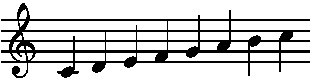
\includegraphics[width=0.8\textwidth]{examples/04theory/01-scale.cropped.pdf}
      \end{center}
      \caption[The \musPitch{C}{}-major scale written in the treble clef.]{The \musPitch{C}{}-major scale written in the treble clef. \examplelink.}
      \label{fig:c-major-scale}
    \end{example}

    % Eb major scale
    \begin{example}[H]
      \begin{center}
        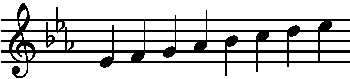
\includegraphics[width=0.8\textwidth]{examples/04theory/02-scale_eb.cropped.pdf}
      \end{center}
      \caption[The \musPitch{E\fl}{}-major scale written in the treble clef.]{The \musPitch{E\fl}{}-major scale written in the treble clef. \examplelink.}
      \label{fig:eb-major-scale}
    \end{example}

    The concept of a musical key is simply shifting where the tonic note is placed. For instance, in Example~\ref{fig:c-major-scale} you can see the major scale in \musPitch{C}{}, and Example~\ref{fig:eb-major-scale} shows the major scale in \musPitch{E\musFlat}{}. These two scales preserve the same intervallic relationships even though the actual pitches are different. The key is simply named after the tonic note, so the first example is in the key of \musPitch{C}{} major and the second example is in the key of \musPitch{E\fl}{} major. The concept of a key is important because it gives us a reference point for understanding the function of notes and chords within a piece of music. It also helps us understand how melodies and harmonies are constructed and how they relate to each other.

  % \subsection{Melodies}
  %   Melodies is the horizontal component of music, meaning we look at it as a time-series. We have a given note at a given length followed by another note or rest of a given length etc... This means that you can look at a melody as a series of intervals as well. If we do this on known melodies we will observe that they are mainly composed of steps and skips. This means that the distance between one note and the next is one or two tones. Large leaps are usually leaping to important tones like the tonic or the root of the current chord. 

  \subsection{Intervals}
    Before discussing harmony we need to consider the different types of distances between notes. The musical distance between two notes is called an \textit{interval}. Intervals can be identified by the number of semitones between the notes. All intervals have special names, and some distances can have different names depending on how they are spelled\footnote{the same pitch can be "spelled" in different ways, for instance \musPitch{A\fl}{} and \musPitch{G\musSharp}{} are written differently, but sound the same since they are the same pitch}. These names can be seen in Table~\ref{tab:intervals}, which also provides the number of semitones between the notes.

    In Figure~\ref{fig:normal_intervals} we can see how all the normal intervals look on a stave. Naming the interval starts by finding the general distance, meaning we first look at the note names. If we consider the interval between \musPitch{C}{} and \musPitch{E\fl}{}, we first observe that from \musPitch{C}{} to \musPitch{E}{} we count three letter names: \musPitch{C}{}, \musPitch{D}{}, and \musPitch{E}{}. This means we have some kind of third. We then look at the quality of that third. Since the \musPitch{E}{} is flattened to \musPitch{E\fl}{}, we have a minor third because the distance is 3 semitones instead of 4. You can see this in Example~\ref{fig:all_intervals}. There we observe that the distance between the notes in a minor third and a major third is the same in terms of letter names; the only difference is that the minor third is one semitone smaller, and that is shown by the \musFlat{}-symbol. Consequently, for the tritone we see that there are two ways to spell the same sounding interval: one is a fourth that has been raised and the other is a fifth that has been lowered. These two are \textit{enharmonically equivalent}, which means that they sound the same even though they are spelled differently. For the augmented fourth, which is the first spelling of the tritone shown here, we see the \musSharp{}-symbol used to indicate that the note has been raised by a semitone.


    \begin{table}
      \caption{Table containing all musical intervals up to an octave, the number of semitones and their abbreviated form.}\label{tab:intervals}
      \begin{center}
        \begin{tabular}[c]{|l|l|l|}
          \hline
          \multicolumn{1}{|c|}{\textbf{Interval name}} & 
          \multicolumn{1}{c|}{\textbf{Semitones}} &
          \multicolumn{1}{c|}{\textbf{Abbreviation}} \\
          \hline
          Unison & 0 & P1\\
          Minor second & 1 & m2 \\
          Major second & 2 & M2 \\
          Minor third & 3 & m3 \\
          Major third & 4 & M3 \\
          Perfect fourth & 5 & P4 \\
          Tritone\tablefootnote{can also be called diminished fifth or augmented fourth, where diminished simply means lowered by semitone and augmented means raised by one semitone} & 6 & TT or aug4/dim5\\
          Perfect fifth & 7 & P5 \\
          Minor sixth & 8 & m6 \\
          Major sixth & 9 & M6 \\
          Minor seventh & 10 & m7 \\
          Major seventh & 11 & M7 \\
          Octave & 12 & P8 \\
          
          \hline
        \end{tabular}
      \end{center}
    \end{table}

    \begin{figure}[H]
      \begin{center}
        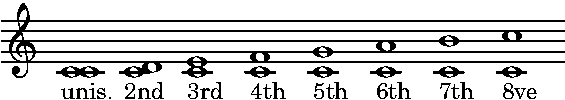
\includegraphics[width=0.95\textwidth]{examples/04theory/03-normal_intervals.cropped.pdf}
      \end{center}
      \caption{All normal intervals from the note \musPitch{C}{4} devoid their variants in quality.}\label{fig:normal_intervals}
    \end{figure}

    \begin{example}[H]
      \begin{center}
        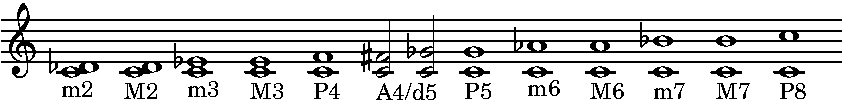
\includegraphics[width=0.95\textwidth]{examples/04theory/04-all_intervals.cropped.pdf}
      \end{center}
      \caption[All musical intervals from the unison to the octave, including their variants.]{All the musical intervals from the unison to the octave including their variants. \examplelink.}\label{fig:all_intervals}
    \end{example}
    
  \subsection{Harmony}\label{sec:harmony}
    Harmony is the vertical component of the music, meaning the notes that happen at the same time. When more than one note is played at the same time we call them chords.
    When considering harmonic progression in tonal music we can consider all the standard chords in the major key. They are labelled by Roman numerals. Upper case means the chord is major and lower case means it is minor. You can see the difference between major and minor chords in Example~\ref{fig:four_chords}, and hear the difference through the link provided in the caption. \\

    Example~\ref{fig:diatonic_chords_d_major} shows the full set of diatonic triads in D major\footnote{the $vii\deg$ means that it is a diminished chord, explanation can be seen in Figure~\ref{fig:four_chords}}. The Roman numerals make the chord quality clear, and the functional labels connect each triad to its role in the key. This is the harmonic material that forms the basis for the progression patterns discussed below.

    \begin{example}[h]
      \begin{center}
        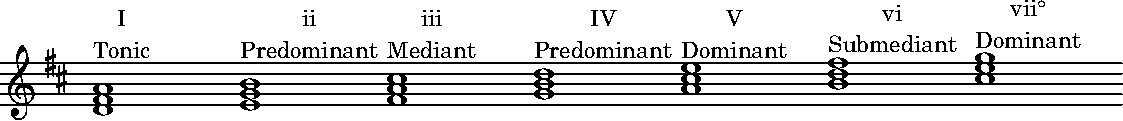
\includegraphics[width=0.98\textwidth]{examples/04theory/11-diatonic_chords.cropped.pdf}
      \end{center}
      \caption[The diatonic triads in D major with Roman numerals and functional names.]{The diatonic triads in D major with Roman numerals and functional names. \examplelink.}\label{fig:diatonic_chords_d_major}
    \end{example}

    Looking at Figure~\ref{fig:harmonic_progression} we can see the typical flow of harmonic functions in tonal music. Tonic means the home, the most stable function. Dominant is the function with the most tension. Pre-dominant usually leads into the dominant or sets the expectation for the dominant. The mediant and submediant are usually not considered part of the main harmonic progression, but they can be used to create interesting harmonic progressions and add some colour to the music. The arrows indicate the typical flow of harmonic functions, however this is not a strict rule. \\

    In harmonic context we often talk about cadences. Cadences classify how one harmony moves into another. The most common cadence is the \ac{PAC}, where we move from the dominant function to the tonic function, for instance from V to I. This is the most stable and resolved cadence, and it is the musical equivalent of a full stop in language. A closely related cadence is the \ac{IAC}, which also moves from dominant to tonic, but lacks some part of the full closure of a \ac{PAC}, for instance because the soprano does not end on the tonic or because one of the chords is inverted. Another common cadence is the \ac{HC}, where the phrase ends on the dominant, for instance by moving from IV to V. This creates tension and leaves us hanging on the dominant function, which usually leads back to the tonic. There are many other types of cadences, but these are among the most common ones. \cite{benCadencesMusicTheory2013} \\

    When writing music with harmonization we often restrict the individual melodies to certain ranges. This ensures that if the music is to be sung or played, the performer must be able to reach all the notes in the line. In traditional four-part harmony, the human voice is often used as the reference instrument, and the different vocal ranges have different names. From the highest voice to the lowest we have the \textit{soprano}, \textit{alto}, \textit{tenor}, and \textit{bass}. The soprano and alto voices are usually female voices, while the tenor and bass voices are usually male voices.
    When writing a harmonization we specify which voices are present. For instance, we can have an SATB harmonization, meaning all four standard voice types are present. We can also have TTBB, which means we have two tenor voices and two bass voices. This concept will be used when the generated melodies are harmonized later in the thesis.

    \begin{figure}[h]
      \centering
      \begin{tikzpicture}[
        node distance=1.8cm,
        every node/.style={font=\large},
        arrow/.style={-Latex, thick},
        box/.style={draw, thick, inner sep=6pt}
        ]

        % Main nodes
        \node (iii) {iii};
        \node[right=of iii] (vi) {vi};

        \node[right=of vi] (pre) {
            \begin{tabular}{c}
              ii\\
              IV
            \end{tabular}
          };

        \node[right=of pre] (dom) {
            \begin{tabular}{c}
              V\\
              vii$^\circ$
            \end{tabular}
          };

        \node[right=of dom] (I) {I};
        \node[right=0.8cm of I] (any) {ANY};
        
        \node[above=24pt of I] {\small Tonic};
        \node[above=24pt of iii] {\small Mediant};
        \node[above=24pt of vi] {\small Submediant};

        % Boxes around functional groups
        \node[box, fit=(pre)] (prebox) {};
        \node[above=4pt of prebox] {\small Pre-dominant};

        \node[box, fit=(dom)] (dombox) {};
        \node[above=4pt of dombox] {\small Dominant};

        % Arrows (horizontal)
        \draw[arrow] (iii) -- (vi);
        \draw[arrow] (vi) -- (prebox);
        \draw[arrow] (prebox) -- (dombox);
        \draw[arrow] (dombox) -- (I);
        \draw[arrow] (I) -- (any);

        % Curved return arrow
        \draw[arrow] 
          (dombox.south) 
          .. controls +(0,-1.5) and +(0,-1.5) .. 
          (iii.south);

      \end{tikzpicture}
      \caption{Harmonic progression in tonal music. The arrows indicate the typical flow of harmonic functions.}\label{fig:harmonic_progression}
    \end{figure}

    \begin{example}[h]
      \begin{center}
        
\includegraphics[width=0.95\textwidth]{examples/04theory/10-majmin.cropped.pdf}
      \end{center}
      \caption[The four main triads: major, minor, diminished, and augmented.]{The four main triads (chords with three notes): major, minor, diminished, and augmented. These are the most basic chord qualities, but major and minor are the most common ones. \examplelink.}\label{fig:four_chords}
    \end{example}
    
  \pagebreak{}
  \subsection{Time signatures}
    The time signature in a piece of music explains the temporal aspect, meaning it dictates how many of which duration fits into a single bar of music. A bar is the space between the vertical lines on the staff.
    A $4/4$ time signature, sometimes written as \meterC, means that there are four quarter notes per bar, and consequently $3/4$ time means that there are three quarter notes per bar. For this thesis I will only employ the standard $4/4$ time signature; it is the most common and straightforward time signature. Figure~\ref{fig:timesignatures} shows a few common time signatures. Notice how $4/4$ and $2/2$ contain the same total amount of time per bar, but the note values are grouped differently. This distinction affects how the music is subdivided and consequently how the rhythm is perceived and felt.

    \begin{figure}[H]
      \begin{center}
        
\includegraphics[width=0.95\textwidth]{examples/04theory/07-timesigs.cropped.pdf}
      \end{center}
      \caption{Demonstration of a few common time signatures and how the type of note is the lower number and the amount is the higher. For instance, $\frac{3}{4}$ has \textit{three} instances of the \textit{quarter} note. }\label{fig:timesignatures}
    \end{figure}

  \subsection{Musical form}
    Now that we have an idea of the musical structures on the melodic and harmonic layer we will take a look at musical forms. This is a very important idea when it comes to constructing melodies. A melody is not an infinitely wandering idea of music. A good melody follows a form. Often this can be viewed as repetitions and variations of a given musical idea. Two very common forms of musical form are the \textit{sentence form} and the \textit{period form}. \cite[pp.20-24]{shoenbergComposition}

    In Example~\ref{fig:sentence} we can see an example of the musical sentence. It starts with a 2-bar opening phrase labelled as the \textit{basic idea}, then we have a repetition of the same idea adapted to a new chord. The following 2 bars are a fragmentation of the idea. The last two bars form a conclusion, which ties the idea together. The cadence at the end can be considered the end of the sentence before the music moves on to something else.

    \begin{example}[H]
      \begin{center}
        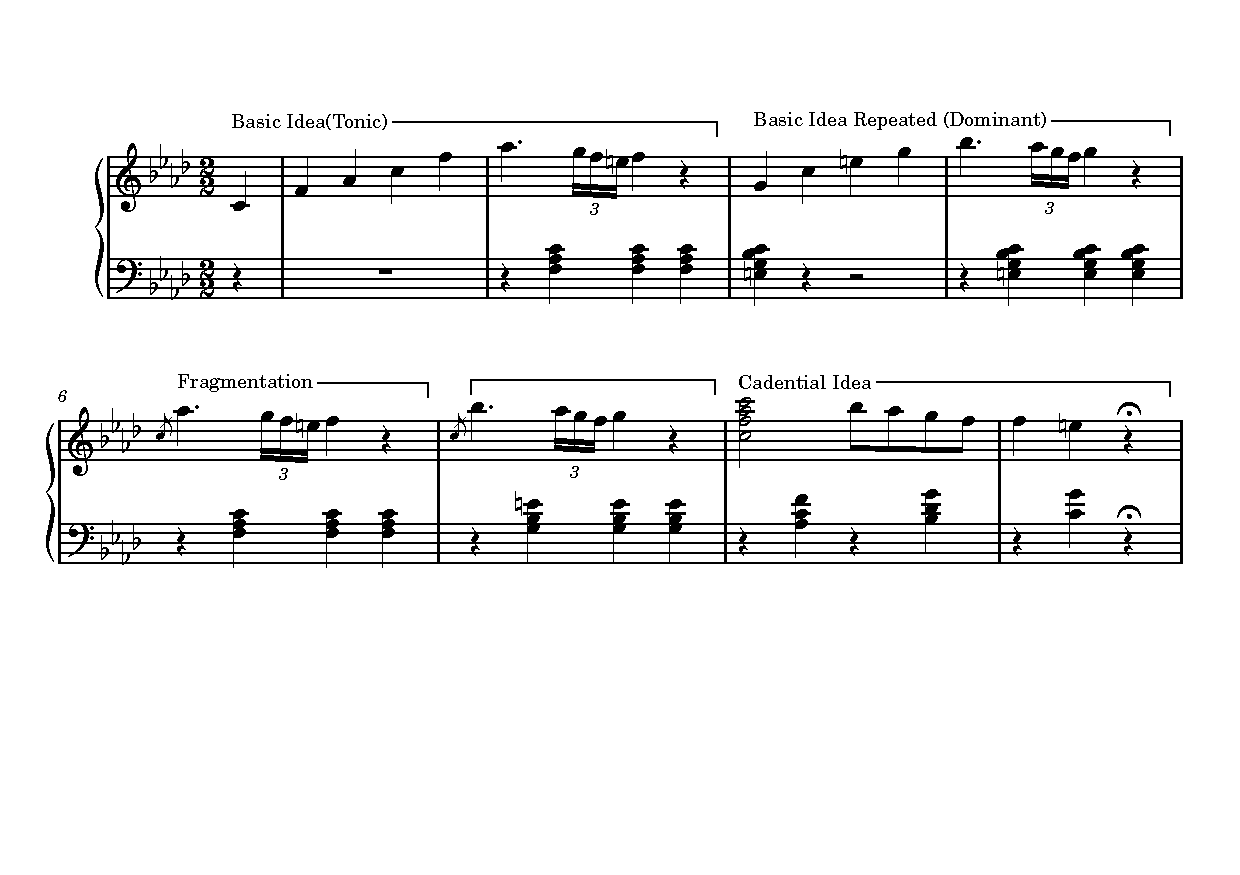
\includegraphics[width=1\textwidth]{examples/04theory/musical_sentence.cropped.pdf}
      \end{center}
      \caption[A classical example of the musical sentence form from the opening bars of Beethoven's piano sonata in F minor.]{A classical example of the musical sentence form. These are the opening bars of Beethoven's piano sonata in F minor \cite{SentenceMusic2023}. \examplelink}\label{fig:sentence}
    \end{example}

    In Example~\ref{fig:period} we see an example of the musical period. This example is from the British folk song \textit{Greensleeves}. The period is a form that is very similar to the sentence, but it has a more balanced structure. It consists of two phrases: the first one is called the \textit{antecedent} and the second one the \textit{consequent}. The antecedent phrase ends with a half cadence, which creates tension and leads us to the consequent phrase, which ends with a perfect authentic cadence and gives us a sense of closure\footnote{see Section~\ref{sec:harmony} for recap of cadences}.

    \begin{example}[H]
      \begin{center}
        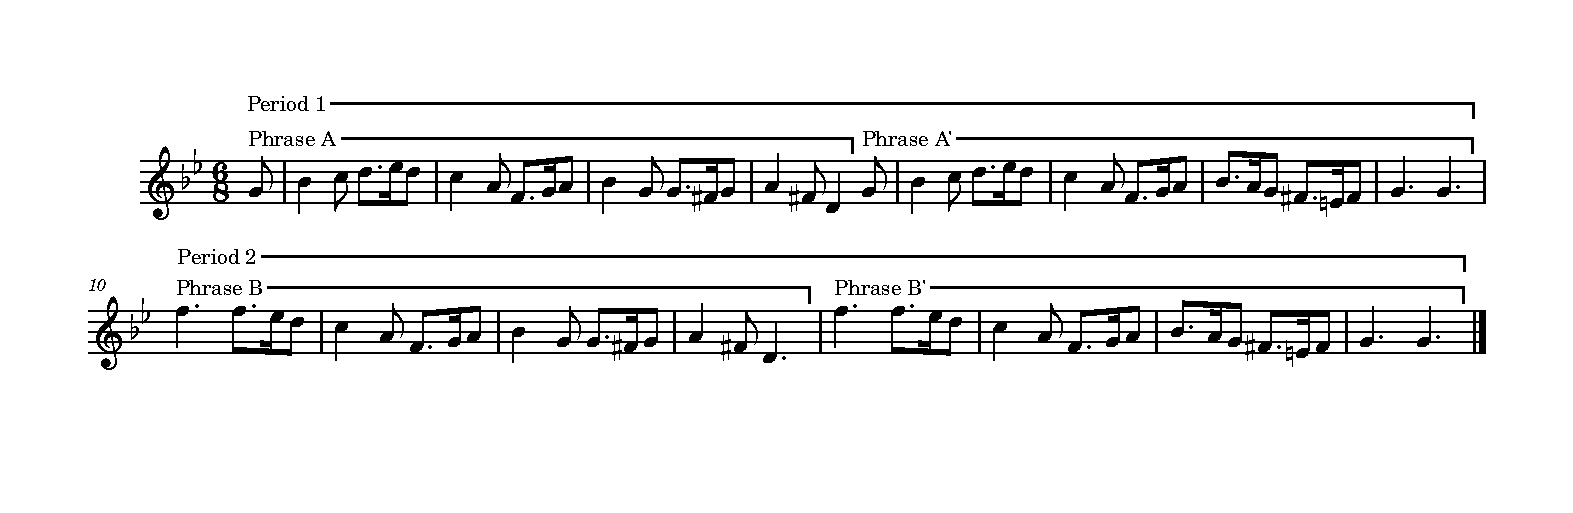
\includegraphics[width=1\textwidth]{examples/04theory/musical_period.cropped.pdf}
      \end{center}
      \caption[A classical example of the musical period form from the melody of the British folk song \textit{Greensleeves}.]{A classical example of the musical period form. This is the melody of the British folk song \textit{Greensleeves} \cite{PeriodMusic2025}. \examplelink}\label{fig:period}
    \end{example}
